\documentclass{article}
\usepackage[utf8]{vietnam}
\usepackage{amsmath}
\usepackage{graphicx}
\graphicspath{ {} }

\title{test}
\author{Nguyễn Tiến Hoàng}
\date{July 2022}

\begin{document}

\maketitle

\section{Lí do sử dụng OOP}
\begin{itemize}
  \item Dễ sửa , phát triển , mở rộng , bảo trì ,  kiểm soát dự án
  \item Dễ đọc code ( giao diện rõ ràng ) , dễ comment , tách file , ...
  \item Sử dụng lại đối tượng , tiết kiệm tài nguyên
  \item Đảm bảo nhất quán dữ liệu và rằng buộc
  \item Kết hợp rất tốt với DB
  \item Ánh xạ trực tiếp thế giới thật
  \item Mô hình hóa những thứ phức tạp dưới dạng cấu trúc đơn giản.
  \item DataStructrue và Algorithms tách rời nhau
  \item Các đối tượng che dấu dữ liệu và truy cập với nhau bằng cách gửi thông điệp ( messages ) thông qua Interface ( Methods )
        \hfill \break \break -> Tiết kiệm chi phí , thời gian , Nâng cao chất lượng
\end{itemize}

\section{Các Thuộc tính của Hướng đối tượng}
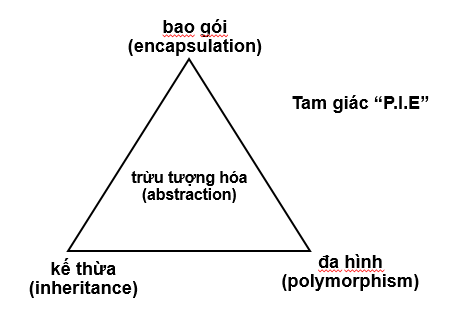
\includegraphics{PIE}
\begin{itemize}
  \item Đóng gói
        \begin{itemize}
          \item Che dấu thông tin và xử lý bên trong của đối tượng
          \item Thao tác đối tượng phải thông qua Interface không làm thay đổi trạng thái của đối tượng
          \item Nhất quán những thành phần bên trong đối tượng , Dễ dàng sử dụng lại
        \end{itemize}
        \break
        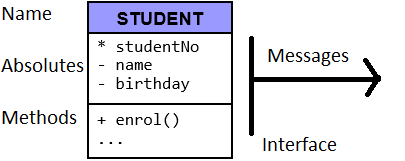
\includegraphics{Object}
        \break
  \item Kế thừa
        \begin{itemize}
          \item dẫn xuất methods + absolutes của lớp cơ sở
          \item kế thừa các đối tượng tổng quát rồi chuyên biệt hóa
          \item Tăng tính logic và tiết kiệm tài nguyên
        \end{itemize}
  \item Đa hình
        \begin{itemize}
          \item Đa dạng hình thức thể hiện của lớp cơ sở
          \item Cùng một phương thức , nhưng cách thức hoạt động của các lớp con có thể khác nhau
        \end{itemize}
  \item Trừu tượng hóa
        \begin{itemize}
          \item loại bỏ những thứ phức tạp, không cần thiết của đối tượng và chỉ tập trung vào những gì cốt lõi, quan trọng.
        \end{itemize}
\end{itemize}

\section{Kiểm soát truy cập}
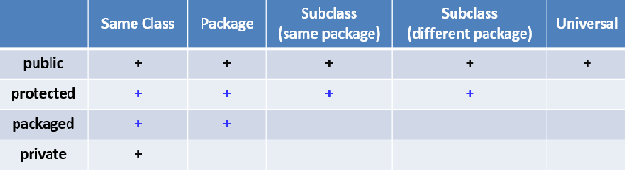
\includegraphics{ConnectionControl}

\section{Các loại lập trình để so sánh với OOP}
\begin{itemize}
  \item Không cấu trúc
  \item Có cấu trúc ( thủ tục )
  \item Logic
  \item Hàm
  \item OOP
\end{itemize}

\section{Các câu hỏi khả năng cao xuất hiện trong đề thi}
\begin{itemize}
  \item Nêu các thuộc tính của LT hướng đối tượng ?
  \item Lí do lập trình HDT ?
  \item So sánh LT Hướng đối tượng với Các hình thức LT khác
  \item Garbage Collection
\end{itemize}


\end{document}
